%%%%%%%%%%%%%%%%%%%%%%%%%%%%%%%%%%%%%%%%%%%%%%%%%%%%%%%%%%%%%%%%
%%%%%%%%%%%%%%%%%%%%%%%%%%%%%%%%%%%%%%%%%%%%%%%%%%%%%%%%%%%%%%%%
\section{Count data models}
\label{sec:countDataModels}


%%%%%%%%%%%%%%%%%%%%%%%%%%%%%%%%%%%%%%%%%%%%%%%%%%%%%%%%%%%%%%%%
\subsection{Homogenous Poisson model -- PM}
\label{subsec:PMmodel}

\paragraph{Observation model}

\begin{itemize}
\item
Type of observed variable -- discrete/count
\item
Model name: Homogenous Poisson process
\item
Count variable: $y$
\item
Probability mass function (PMF)
\begin{eqnarray}
&& P(y=k; \lambda) = \frac{\lambda^k \exp(-\lambda)}{k!} \nonumber
\end{eqnarray}
\item
Link function: $\log$
\item
Constant rate parameter $\lambda$ -- \emph{homogenous Poisson process}:
\begin{eqnarray}
&& \lambda(t_{ij}, \psi_{ij}) = \lambda_{i} \nonumber
\end{eqnarray}
\end{itemize}


\paragraph{Individual parameter model}
\begin{eqnarray}
\lambda & \sim& \mbox{logNormal}(\lambda_{\rm pop}, \omega_{\lambda});  \quad \lambda_{\rm pop}=1,\quad \omega_{\lambda}=0.6 \nonumber
\end{eqnarray}


%\begin{center}
%\begin{longtable}{lll}
%\hline
%\hline
%\pml element 			&  version $\le$ 0.3.1 					& version 0.4 \\
%or modelling aspect 		&								& \\
%\hline
%Delay differential equations (DDE) 	& \emph{not supported}		& \xelem{Delay} and \xelem{History}  \\
%(see \textsection\ref{sec:DDmodels})	& 					& the latter with child elements \\ 
%						&							& -- \xelem{HistoryValue} and \\
%						&							& -- \xelem{HistoryTime} {\color{red} \scshape{new}} \\ 
%\hline
%Extended matrix and vector support & supported but			&  ... \\
%						& without indexing 				& \\
%\hline
%%row1						&  ... \\
%\hline
%\caption{Overview of major differences between versions 0.4 and 0.3.1}
%\label{figTable:overviewTable}
%\end{longtable}
%\end{center}


%\begin{center}
%\begin{longtable}{lll}
%\hline
%\end{longtable}
%\end{center}

\subsubsection{NM-TRAN code:}
Code provided by Elodie Plan.

\myStartLine

%\lstset{language=MLXTRANcode}
\lstset{language=NONMEMdataSet}
\begin{lstlisting}
$PROB Poisson distribution function 
$DATA data.csv IGNORE=@ 
$INPUT ID TIME DV

$PRED 
; Parameters
 LAMB=THETA(1)*EXP(ETA(1))

; Factorial approximation 
 IF(DV.LE.1) THEN
     LFAC=0 
     ELSE 
     LFAC = DV*LOG(DV)-DV + LOG(DV*(1+4*DV*(1+2*DV)))/6 +LOG(3.1415)/2
 ENDIF

; Likelihood definition  
 LPOIS = -LAMB+DV*LOG(LAMB)-LFAC 
 Y = -2*LPOIS

; Simulation code 
 IF (ICALL.EQ.4) THEN
     LAMB=THETA(1)*EXP(ETA(1)) 
     T=0 
     N=0 
     DO WHILE (T.LT.1)
          CALL RANDOM (2,R) 
          T=T-LOG(1-R)/LAMB 
          IF (T.LT.1) N=N+1
     END DO
     DV=N 
ENDIF

$THETA (0,0.5)             ; LAMBDA

$OMEGA 0.1

$ESTIMATION MAXEVAL=9999 METHOD=COND LAPLACE -2LL 
$COV 
;$SIMULATION (361734) (474980 UNIFORM) ONLYSIM NOPRED 
$TABLE ID TIME DV NOAPPEND ONEHEADER NOPRINT FILE = tab
\end{lstlisting}

\myEndLine

\subsubsection{MLXTRAN code:}
Based on from Monolix 4.1.4 User Guide \cite{Monolix4.1.4UserGuide:2012}

\myStartLine

\lstset{language=MLXTRANcode}
\begin{lstlisting}
DESCRIPTION:
Poisson model

DATA:
modelFile='pkcount.txt';
modelPath='../../models/pkpd_models';

INDIVIDUAL:
lambda = {distribution=logNormal, iiv=yes}

pop_lambda = 0.5;     omega_lambda = 0.1;

OBSERVATION:
Y = {
      type = count
      Log(P(Y=k)) = -lambda + k*log(lambda) - factln(k)
}

OUTPUT: 
output = Y
\end{lstlisting}

\myEndLine


The following code assumes that the intensity parameter of the Possion distribution, $lambda$, 
is defined in the \xelem{ParameterModel  blkId="pm1"}.

\subsubsection{PharmML code -- Version 1:}
Using log-PMF

\lstset{language=XML}
\begin{lstlisting}				
        <ObservationModel blkId="om1">
            <Discrete>
                <CountData>
                    <CountVariable symbId="Y"/>
                    <IntensityParameter symbId="Lambda">
                        <ct:Assign>
                            <ct:SymbRef blkIdRef="pm1" symbIdRef="lambda"/>
                        </ct:Assign>
                    </IntensityParameter>
                    
                    <!-- log(P(Y=k)) = -Lambda+k*log(Lambda)-log(k!) -->
                    <PMF linkFunction="log">
                        <math:LogicBinop op="eq">
                            <ct:SymbRef symbIdRef="Y"/>
                            <ct:SymbRef symbIdRef="k"/>
                        </math:LogicBinop>
                        <ct:Assign>
                            <Equation xmlns="http://www.pharmml.org/2013/03/Maths">
                                <Binop op="minus">
                                    <Binop op="plus">
                                        <Uniop op="minus">
                                            <ct:SymbRef symbIdRef="Lambda"/>
                                        </Uniop>
                                        <Binop op="times">
                                            <ct:SymbRef symbIdRef="k"/>
                                            <Uniop op="log">
                                                <ct:SymbRef symbIdRef="Lambda"/>
                                            </Uniop>
                                        </Binop>
                                    </Binop>
                                    <Uniop op="factln">
                                        <ct:SymbRef symbIdRef="k"/>
                                    </Uniop>
                                </Binop>
                            </Equation>
                        </ct:Assign>
                    </PMF>
                </CountData>
            </Discrete>
        </ObservationModel>
\end{lstlisting}

\subsubsection{Version 2}
Now using the untransformed PMF and UncertML.

\lstset{language=XML}
\begin{lstlisting}				
        <ObservationModel blkId="om1">
            <Discrete>
                <CountData>
                    <CountVariable symbId="Y"/>
                    
                    <IntensityParameter symbId="Lambda">
                        <ct:Assign>
                            <ct:SymbRef blkIdRef="pm1" symbIdRef="lambda"/>
                        </ct:Assign>
                    </IntensityParameter>
                    
                    <PMF>
                        <PoissonDistribution xmlns="http://www.uncertml.org/3.0" 
                        definition="http://www.uncertml.org/3.0">
                            <rate>
                                <var varId="Lambda"/>
                            </rate>
                        </PoissonDistribution>
                    </PMF>
                </CountData>
            </Discrete>
        </ObservationModel>
\end{lstlisting}


%%%%%%%%%%%%%%%%%%%%%%%%%%%%%%%%%%%%%%%%%%%%%%%%%%%%%%%%%%%%%%%
\subsection{Poisson model with Markovian dependence -- PMAK}
\label{subsec:PMAKmodel}

\paragraph{Observation model}

\begin{itemize}
\item
Type of observed variable -- discrete/count
\item
Model name: Homogenous Poisson process
\item
Count variable: $y$
\item
Previous state variable: $yp$
\item
Probability mass function with Markov dependance which can be formulated in
two ways
\begin{itemize}
\item
(version 1) using conditional statement for the $\lambda$'s and one PMF definition
\begin{align}
 \lambda = \left\{ \begin{array}{rcl}
			\lambda_1 & \mbox{for} & yp = 0 \\
			\lambda_2 & \mbox{for} & yp \neq 0 \nonumber
\end{array}\right. 
\quad \text{and} \quad P(y=k; \lambda) = \frac{\lambda^k \exp(-\lambda)}{k!} \nonumber
\end{align}
\item
(version 2) or define the PMF's separately 
\begin{align}
& P(y=k | yp=0; \lambda_1) = \frac{\lambda_1^k \exp(-\lambda_1)}{k!} \nonumber \\
& P(y=k | yp \neq 0; \lambda_2) = \frac{\lambda_2^k \exp(-\lambda_2)}{k!} \nonumber 
\end{align}
\end{itemize}
\item
Link function: $\log$
\item
Constant rate parameters $\lambda_1,\lambda_2$ -- \emph{homogenous Poisson process}:
\begin{eqnarray}
& \lambda(t_{ij}, \psi_{ij}) = \lambda_{1/2,i} \nonumber
\end{eqnarray}
\end{itemize}


\subsubsection{NM-TRAN code provided by Elodie Plan:}

\myStartLine

\lstset{language=NONMEMdataSet}
\begin{lstlisting}
$PROB Poisson distribution function with Markov component
$DATA data.csv IGNORE=@
$INPUT ID TIME DV PDV  ;PDV = previous DV = 0 or more here

$PRED
; Parameters
              LAMB=THETA(1)*EXP(ETA(1))
 IF(PDV.EQ.0) LAMB=THETA(2)*EXP(ETA(2))

; Factorial approximation
 IF(DV.LE.1) THEN
    LFAC=0
    ELSE
    LFAC = DV*LOG(DV)-DV +LOG(DV*(1+4*DV*(1+2*DV)))/6 +LOG(3.1415)/2
 ENDIF

; Likelihood definition
 LPOIS = -LAMB+DV*LOG(LAMB)-LFAC
 Y = -2*LPOIS

; Simulation code
    IF(NEWIND.NE.2) PPSDV=1
    IF(NEWIND.NE.2) PSDV=1
    PPSDV=PSDV
    PDV=PSDV

    IF (ICALL.EQ.4) THEN
                     LAMB=THETA(1)*EXP(ETA(1))
       IF(PSDV.EQ.0) LAMB=THETA(2)*EXP(ETA(2))
       T=0
       N=0
       DO WHILE (T.LT.1)
            CALL RANDOM (2,R)
            T=T-LOG(1-R)/LAMB
            IF (T.LT.1) N=N+1
       END DO
       DV=N
    ENDIF

    PSDV=0
    IF(DV.GE.1) PSDV=1

$THETA (0,0.65)       ; LAMBDA 1
$THETA (0,0.40)       ; LAMBDA 2

$OMEGA BLOCK(2)
0.91 
0.62 0.76

$ESTIMATION MAXEVAL=9999 METHOD=COND LAPLACE -2LL
$COV
;$SIMULATION (361734) (474980 UNIFORM) ONLYSIM NOPRED
$TABLE ID TIME DV PDV NOAPPEND ONEHEADER NOPRINT FILE = tab

\end{lstlisting}

\myEndLine

\subsubsection{MLXTRAN code by MS and Mark Lavielle:}

\myStartLine

\lstset{language=MLXTRANcode}
\begin{lstlisting}
DESCRIPTION:
Poisson model with Markovian dependence,

DATA:
modelFile='pkcount.txt';
modelPath='../../models/pkpd_models';

INDIVIDUAL:
lambda1 = {distribution=logNormal, iiv=yes}
lambda2 = {distribution=logNormal, iiv=yes}

pop_lambda1 = 0.64;     omega_lambda1 = 0.91;
pop_lambda2 = 0.40;     omega_lambda2 = 0.76;
rho_lambda1_lambda2 = 0.62

EQUATION:
if Yp==0
     lambda=lambda1
else
     lambda=lambda2
end

OBSERVATION:
Y = {
      type = count
      Log(P(Y=k)) = -lambda + k*log(lambda) - factln(k)
}

OUTPUT: 
output = Y
\end{lstlisting}

\myEndLine

The following \pharmml implementations assume that the parameters \emph{lambda1} 
and \emph{lambda2}, with inter-individual variability, are defined in the parameter 
model \xatt{pm1}.

\subsubsection{PharmML code -- version 1:}
This version applies the conditional statement as in the MLXTRAN code above 
-- see an alternative implementation in next section. 

\lstset{language=XML}
\begin{lstlisting}	
        <ObservationModel blkId="om1">
            <Discrete>
                <CountData>
                    <CountVariable symbId="y"/>
                    <PreviousCountVariable symbId="yp"/>
                    
                    <Dependance type="discreteMarkov"/>
                    
                    <!-- Version 1 -->
                    <!-- Poisson with Markov - choose one lambda dependent on yp -->
                    <IntensityParameter symbId="Lambda">
                        <ct:Assign>
                            <math:Equation>
                                <math:Piecewise>
                                    <math:Piece>
                                        <ct:SymbRef blkIdRef="pm1" symbIdRef="lambda1"/>
                                        <math:Condition>
                                            <math:LogicBinop op="eq">
                                                <ct:SymbRef symbIdRef="yp"/>
                                                <ct:Real>0</ct:Real>
                                            </math:LogicBinop>
                                        </math:Condition>
                                    </math:Piece>
                                    <math:Piece>
                                        <ct:SymbRef blkIdRef="pm1" symbIdRef="lambda2"/>
                                        <math:Condition>
                                            <math:Otherwise/>
                                        </math:Condition>
                                    </math:Piece>
                                </math:Piecewise>
                            </math:Equation>
                        </ct:Assign>
                    </IntensityParameter>
                    
                    <!-- log(P(y=k)) = -lambda + k*log(lambda) - factln(k) -->
                    <PMF linkFunction="log">
                        <math:LogicBinop op="eq">
                            <ct:SymbRef symbIdRef="y"/>
                            <ct:SymbRef symbIdRef="k"/>
                        </math:LogicBinop>
                        <ct:Assign>
                            <math:Equation>
                                <math:Binop op="plus">
                                    <math:Uniop op="minus">
                                        <ct:SymbRef symbIdRef="Lambda"/>
                                    </math:Uniop>
                                    <math:Binop op="plus">
                                        <math:Binop op="times">
                                            <ct:SymbRef symbIdRef="k"/>
                                            <math:Uniop op="log">
                                                <ct:SymbRef symbIdRef="Lambda"/>
                                            </math:Uniop>
                                        </math:Binop>
                                        <math:Uniop op="factln">
                                            <ct:SymbRef symbIdRef="k"/>
                                        </math:Uniop>
                                    </math:Binop>
                                </math:Binop>
                            </math:Equation>
                        </ct:Assign>
                    </PMF>
                </CountData>
            </Discrete>
       </ObservationModel>
\end{lstlisting}

%%%%% Version 2 - with Previous/Current-State elements
\subsubsection{PharmML code -- version 2:}
This version uses two \xelem{IntensityParameter} elements, one for the current, one
for the previous state and accordingly two \xelem{PMF} statements using UncertML.
\lstset{language=XML}
\begin{lstlisting}	
        <ObservationModel blkId="om2">
            <Discrete>
                <CountData>
                    <CountVariable symbId="y"/>
                    <PreviousCountVariable symbId="yp"/>
                    
                    <Dependance type="discreteMarkov"/>
                    
                    <!-- Version 2 -->
                    <!-- Poisson with Markov -->
                    <IntensityParameter symbId="Lambda1">
                        <ct:Assign>
                            <ct:SymbRef blkIdRef="pm1" symbIdRef="lambda1"/>
                        </ct:Assign>
                    </IntensityParameter>
                    
                    <IntensityParameter symbId="Lambda2">
                        <ct:Assign>
                            <ct:SymbRef blkIdRef="pm1" symbIdRef="lambda2"/>
                        </ct:Assign>
                    </IntensityParameter>
                    
                    
                    <!-- log(P(y=k | yp=0)) = -lambda1 + k*log(lambda1) - factln(k) -->
                    <PMF linkFunction="log">
                        <CurrentState>
                            <math:LogicBinop op="eq">
                                <ct:SymbRef symbIdRef="y"/>
                                <ct:SymbRef symbIdRef="k"/>
                            </math:LogicBinop>                            
                        </CurrentState>
                        <PreviousState>
                            <math:LogicBinop op="eq">
                                <ct:SymbRef symbIdRef="y"/>
                                <ct:Int>0</ct:Int>
                            </math:LogicBinop>
                        </PreviousState>
                        <PoissonDistribution xmlns="http://www.uncertml.org/3.0" definition="http://www.uncertml.org/3.0">
                            <rate>
                                <var varId="Lambda1"/>
                            </rate>
                        </PoissonDistribution>
                    </PMF>
                    
                    <!-- log(P(y=k | yp != 0)) = -lambda2 + k*log(lambda2) - factln(k) -->
                    <PMF linkFunction="log">
                        <CurrentState>
                            <math:LogicBinop op="eq">
                                <ct:SymbRef symbIdRef="y"/>
                                <ct:SymbRef symbIdRef="k"/>
                            </math:LogicBinop>                            
                        </CurrentState>
                        <PreviousState>
                            <math:LogicBinop op="neq">
                                <ct:SymbRef symbIdRef="y"/>
                                <ct:Int>0</ct:Int>
                            </math:LogicBinop>
                        </PreviousState>
                        <!-- omitted -->
                        <!-- equation analog as above with Lambda2 instead of Lambda1 --> 
                    </PMF>
                    
                </CountData>
            </Discrete>
        </ObservationModel>
\end{lstlisting}


%%%%%%%%%%%%%%%%%%%%%%%%%%%%%%%%%%%%%%%%%%%%%%%%%%%%%%%%%%%%%%%%
%\subsubsection{Poisson model with mixture distribution - PMIX}
%\paragraph{NM-TRAN code provided by Elodie Plan}
%\begin{lstlisting}
%$PROB Poisson distribution function with mixture distribution (for individual observations) 
%$DATA data.csv IGNORE=@ 
%$INPUT ID TIME DV
%
%$PRED 
%; Parameters
%     LAMB1 = THETA(1)*EXP(ETA(1)) 
%     LAMB2 = THETA(2)*EXP(ETA(1)) 
%     MP = THETA(3)
%
%; Factorial approximation 
% IF(DV.LE.1) THEN
%     LFAC=0 
%     ELSE 
%     LFAC = DV*LOG(DV)-DV 
%                    + LOG(DV*(1+4*DV*(1+2*DV)))/6 +LOG(3.1415)/2
%ENDIF
%
%; Likelihood definition 
% P1 = EXP(-LAMB1+DV*LOG(LAMB1)-LFAC) 
% P2 = EXP(-LAMB2+DV*LOG(LAMB2)-LFAC)
%
% PMIX = MP*P1 + (1-MP)*P2 
% Y = -2*LOG(PMIX)
%
%; Simulation code 
%     IF (ICALL.EQ.4) THEN
%          LAMB1 = THETA(1)*EXP(ETA(1)) 
%          LAMB2 = THETA(2)*EXP(ETA(1)) 
%          MP = THETA(3) 
%          PN=0
%          N=0 
%          CALL RANDOM (2,R)
%               DO WHILE (PN.LT.R) 
%                     IF(N.LE.1) THEN
%                          LFAC=0 
%                          ELSE 
%                          LFAC = N*LOG(N)-N 
%                                         + LOG(N*(1+4*N*(1+2*N)))/6 +LOG(3.1415)/2
%                     ENDIF 
%                     P1 = EXP(-LAMB1+N*LOG(LAMB1)-LFAC) 
%                     P2 = EXP(-LAMB2+N*LOG(LAMB2)-LFAC) 
%                     PMIX = MP*P1 + (1-MP)*P2
%                     PN = PMIX+PN 
%                     IF (PN.LT.R) N=N+1
%               END DO
%          DV=N 
%     ENDIF
%
%$THETA (0,0.5)             ; LAMBDA1
%$THETA (0,1)                ; LAMBDA2
%$THETA (0,0.5,1)         ; MP
%
%$OMEGA 
% 0.1
%
%$ESTIMATION MAXEVAL=9999 METHOD=COND LAPLACE -2LL 
%$COV 
%;$SIMULATION (361734) (474980 UNIFORM) ONLYSIM NOPRED 
%$TABLE ID TIME DV NOAPPEND ONEHEADER NOPRINT FILE = tab
%\end{lstlisting}
%\paragraph{MLXTRAN code by MS and Mark Lavielle}
%\begin{lstlisting}
%DESCRIPTION:
%Poisson model with mixture distribution
%
%DATA:
%modelFile='pkcount.txt';
%modelPath='../../models/pkpd_models';
%
%INDIVIDUAL:
%lambda1 = {distribution=logNormal, iiv=yes}
%lambda2 = {distribution=logNormal, iiv=yes}
%MP = {distribution=logNormal, iiv=no}
%
%pop_lambda1 = 0.5;    omega_lambda1 = 0.1;
%pop_lambda2 = 1;       omega_lambda2 = 0.1;
%pop_MP = 0.5;
%
%OBSERVATION:
%Y = {
%      type = count
%      P1 = - lambda1 + k*log(lambda1) - factln(k)
%      P2 = - lambda2 + k*log(lambda2) - factln(k)
%      Log(P(Y=k)) = MP*P1 + (1-MP)*P2
%}
%
%OUTPUT: 
%output = Y
%\end{lstlisting}


%%%%%%%%%%%%%%%%%%%%%%%%%%%%%%%%%%%%%%%%%%%%%%%%%%%%%%%%%%%%%%%
\subsection{Negative Binomial model -- NB}
\label{subsec:NBmodel}

\paragraph{Observation model}

\begin{itemize}
\item
Type of observed variable -- discrete/count
\item
Model name: Negative Binomial
\item
Count variable: $y$
\item
Probability mass function
\begin{eqnarray}
P(y_{ij} = k; \lambda, \tau) &=& \Bigg[ \frac{\Gamma \big( k + \frac{1}{\tau} \big)}{k! \times \Gamma \big(\frac{1}{\tau} \big)} \Bigg] \times \Bigg( \frac{1}{1 + \tau \times \lambda} \Bigg)^{\frac{1}{\tau}} \times \Bigg(\frac{\lambda}{\frac{1}{\tau} + \lambda} \Bigg)^k \nonumber
\end{eqnarray}
\item
Link function: $\log$
\item
Dispersion parameter, $\tau$
\item
Constant rate parameter $\lambda$, the Poisson 'intensity': 
\begin{eqnarray}
&& \lambda(t_{ij}, \psi_{ij}) = \lambda_{i} \nonumber
\end{eqnarray}
\end{itemize}


\paragraph{Individual parameter model}
\begin{eqnarray}
\lambda & \sim& \mbox{logNormal}(\lambda_{\rm pop}, \omega_{\lambda});  \quad \lambda_{\rm pop}=0.5,\quad \omega_{\lambda}=0.1 \nonumber \\
\tau & \sim& \mbox{logNormal}(\tau_{\rm pop}, \omega_{\tau});  \quad \tau_{\rm pop}=0.25,\quad \omega_{\tau}=0.1 \nonumber
\end{eqnarray}


\subsubsection{NM-TRAN code:}
Code provided by Elodie Plan

\myStartLine

\lstset{language=NONMEMdataSet}
\begin{lstlisting}
$PROB Negative Binomial distribution function 
$DATA data.csv IGNORE=@
$INPUT ID TIME DV

$PRED
; Parameters
              LAMB=THETA(1)*EXP(ETA(1))
              OVDP=THETA(2)*EXP(ETA(2))

; Factorial approximation
 IF(DV.LE.1) THEN
    LFAC=0
    ELSE
    LFAC = DV*LOG(DV)-DV +LOG(DV*(1+4*DV*(1+2*DV)))/6 +LOG(3.1415)/2
 ENDIF

; Likelihood definition (with Gamma functions approximation)
 LGAM1 = LOG(SQRT(2*3.1415))+((DV+1/OVDP)-0.5)*LOG((DV+1/OVDP)) 
                    -(DV+1/OVDP)+LOG(1+1/(12*(DV+1/OVDP)))
 LGAM2 = LOG(SQRT(2*3.1415))+((1/OVDP)-0.5)*LOG((1/OVDP))
                    -(1/OVDP)+LOG(1+1/(12*(1/OVDP)))

 LTRM1 = (1/OVDP)*LOG(1/(1+OVDP*LAMB))
 LTRM2 = DV*LOG(LAMB/(LAMB+1/OVDP))

 LNB = LGAM1-LFAC-LGAM2+LTRM1+LTRM2

 Y = -2*LNB

; Simulation code (for relatively low OVDP, otherwise switch to non-log 
					expressions for numerical issues)
    IF (ICALL.EQ.4) THEN
       LAMB=THETA(1)*EXP(ETA(1))
       OVDP=THETA(2)*EXP(ETA(2))
       PN=0
       N=0
       CALL RANDOM (2,R)
            DO WHILE (PN.LT.R)
                LGAM1 = LOG(SQRT(2*3.1415))+((N+1/OVDP)-0.5)*LOG((N+1/OVDP))
                                   -(N+1/OVDP)+LOG(1+1/(12*(N+1/OVDP)))
                LGAM2 = LOG(SQRT(2*3.1415))+((1/OVDP)-0.5)*LOG((1/OVDP))
                                   -(1/OVDP)+LOG(1+1/(12*(1/OVDP)))
                LTRM1 = (1/OVDP)*LOG(1/(1+OVDP*LAMB))
                LTRM2 = N*LOG(LAMB/(LAMB+1/OVDP))
                IF(N.LE.1) THEN
                    LFAC=0
                    ELSE
                    LFAC = N*LOG(N)-N +LOG(N*(1+4*N*(1+2*N)))/6 +LOG(3.1415)/2
                ENDIF
                NB = EXP(LGAM1-LFAC-LGAM2+LTRM1+LTRM2)
                PN = NB+PN
                IF (PN.LT.R) N=N+1
          END DO
       DV=N
    ENDIF

$THETA (0,0.50)       ; LAMBDA
$THETA (0,0.25)       ; OVDP

$OMEGA
0.1                   ; LAMBDA
0.1                   ; OVDP

$ESTIMATION MAXEVAL=9999 METHOD=COND LAPLACE -2LL
$COV
;$SIMULATION (361734) (474980 UNIFORM) ONLYSIM NOPRED
$TABLE ID TIME DV NOAPPEND ONEHEADER NOPRINT FILE = tab
\end{lstlisting}

\myEndLine

\subsubsection{MLXTRAN code:}
Code source: Monolix 4.1.4 User Guide \cite{Monolix4.1.4UserGuide:2012}.

\myStartLine

\lstset{language=MLXTRANcode}
\begin{lstlisting}
DESCRIPTION:
Negative Binomial 

DATA:
modelFile='pkcount.txt';
modelPath='../../models/pkpd_models';

INDIVIDUAL:
Ovdp = {distribution=logNormal, iiv=yes}
lambda = {distribution=logNormal, iiv=yes}

pop_Ovdp = 0.25;    omega_Ovdp = 0.1;
pop_lambda = 0.5;   omega_lambda = 0.1;

OBSERVATION:
Y = {
type = count

h1 = 1/(1+lambda*Ovdp) 
llam = log(h1)/Ovdp 
lh2 = log(1-h1)

lg1 = gammaln(k+1/Ovdp) 
lg2 = gammaln(1/Ovdp)

if (k > 0) 
     aux = llam + lg1 - lg2 + k*lh2 - factln(k)
else 
     aux = llam
end 

log(P(Y=k)) = aux
}

OUTPUT: 
output = Y
\end{lstlisting}

\myEndLine

\subsubsection{PharmML code:}
The following code assumes that the parameters $lambda$ and $tau$ are defined in the \xelem{ParameterModel}.

\lstset{language=XML}
\begin{lstlisting}
        <ObservationModel blkId="om1">
            <Discrete>
                <CountData>
                    <!-- y = DV in NMTRAN code -->
                    <CountVariable symbId="y"/>
                    
                    <IntensityParameter symbId="Lambda">
                        <ct:Assign>
                            <ct:SymbRef blkIdRef="pm1" symbIdRef="lambda"/>
                        </ct:Assign>
                    </IntensityParameter>
                    
                    <DispersionParameter symbId="Tau">
                        <ct:Assign>
                            <ct:SymbRef blkIdRef="pm1" symbIdRef="tau"/>
                        </ct:Assign>
                    </DispersionParameter>
                    
                    <PMF linkFunction="log">
                        <!-- log(y=k)  -->
                        <math:LogicBinop op="eq">
                            <ct:SymbRef symbIdRef="y"/>
                            <ct:SymbRef symbIdRef="k"/>
                        </math:LogicBinop>
                        <ct:Assign>
                            <math:Equation>
                                <math:Binop op="minus">
                                    <math:Binop op="plus">
                                        <math:Binop op="minus">
                                            <math:Binop op="minus">
                                                <math:Binop op="minus">
                                                    <!-- gammaln(k+1/tau) -->
                                                    <math:Uniop op="gammaln">
                                                        <math:Binop op="plus">
                                                            <ct:SymbRef symbIdRef="k"/>
                                                            <math:Binop op="divide">
                                                                <ct:Real>1</ct:Real>
                                                                <ct:SymbRef symbIdRef="Tau"/>
                                                            </math:Binop>
                                                        </math:Binop>
                                                    </math:Uniop>
                                                    <!-- factln(k) -->
                                                    <math:Uniop op="factln">
                                                        <ct:SymbRef symbIdRef="k"/>
                                                    </math:Uniop>
                                                </math:Binop>
                                                <!-- gammaln(1/tau) -->
                                                <math:Uniop op="gammaln">
                                                    <math:Binop op="divide">
                                                        <ct:Real>1</ct:Real>
                                                        <ct:SymbRef symbIdRef="Tau"/>
                                                    </math:Binop>
                                                </math:Uniop>
                                            </math:Binop>
                                            <!-- 1/tau log(1+tau * lambda) -->
                                            <math:Binop op="times">
                                                <math:Binop op="divide">
                                                    <ct:Real>1</ct:Real>
                                                    <ct:SymbRef symbIdRef="Tau"/>
                                                </math:Binop>
                                                <math:Uniop op="log">
                                                    <math:Binop op="plus">
                                                        <ct:Real>1</ct:Real>
                                                        <math:Binop op="times">
                                                            <ct:SymbRef symbIdRef="Tau"/>
                                                            <ct:SymbRef symbIdRef="Lambda"/>
                                                        </math:Binop>
                                                    </math:Binop>
                                                </math:Uniop>
                                            </math:Binop>
                                        </math:Binop>
                                        <math:Binop op="times">
                                            <!-- k*log(lambda) -->
                                            <ct:SymbRef symbIdRef="k"/>                         
                                            <math:Uniop op="log">
                                                <ct:SymbRef symbIdRef="Lambda"/>
                                            </math:Uniop>
                                        </math:Binop>
                                    </math:Binop>
                                    <math:Binop op="times">
                                        <!-- k*log(1/tau + lambda) -->
                                        <ct:SymbRef symbIdRef="k"/>                         
                                        <math:Uniop op="log">
                                            <math:Binop op="plus">
                                                <math:Binop op="divide">
                                                    <ct:Real>1</ct:Real>
                                                    <ct:SymbRef symbIdRef="Tau"/>
                                                </math:Binop>
                                                <ct:SymbRef symbIdRef="Lambda"/>
                                            </math:Binop>
                                        </math:Uniop>
                                    </math:Binop>
                                </math:Binop>
                            </math:Equation>
                        </ct:Assign>
                    </PMF>
                </CountData>
            </Discrete>
        </ObservationModel>
    </ModelDefinition>
\end{lstlisting}



%%%%%%%%%%%%%%%%%%%%%%%%%%%%%%%%%%%%%%%%%%%%%%%%%%%%%%%%%%%%%%%
\subsection{Zero inflated model -- ZIP}
\label{subsec:ZIPmodel}

\paragraph{Observation model}

\begin{itemize}
\item
Type of observed variable -- discrete/count
\item
Model name: Zero-inflated
\item
Count variable: $y$
\item
Probability mass function
\begin{align}
& P(y_{ij} = k; \lambda, p_0) =  \left\{ \begin{array}{rcl} p_0 + (1-p_0) e^{-\lambda} & \mbox{if} & k = 0 \\ 
(1-p_0)\frac{e^{-\lambda}\lambda^k}{k!} & \mbox{if} & k > 0 \end{array}\right. \nonumber
\end{align}
\item
Link function: $\log$
\item
Zero probability parameter, $p_0 \in [0,1]$
\item
Constant rate parameter $\lambda$, the Poisson 'intensity': 
\begin{eqnarray}
&& \lambda(t_{ij}, \psi_{ij}) = \lambda_{i} \nonumber
\end{eqnarray}
\end{itemize}

\subsubsection{NM-TRAN code provided by Elodie Plan:}

\myStartLine

\lstset{language=NONMEMdataSet}
\begin{lstlisting}
$PROB Zero-inflated Poisson distribution function
$DATA data.csv IGNORE=@
$INPUT ID TIME DV

$PRED
; Parameters
              LAMB=THETA(1)*EXP(ETA(1))

              LOGIT=LOG(THETA(2)/(1-THETA(2)))
              P0=EXP(LOGIT+ETA(2))/(1+EXP(LOGIT+ETA(2)))

; Factorial approximation
 IF(DV.LE.1) THEN
    LFAC=0
    ELSE
    LFAC = DV*LOG(DV)-DV +LOG(DV*(1+4*DV*(1+2*DV)))/6 +LOG(3.1415)/2
 ENDIF

; Likelihood definition
 LPOIS = -LAMB+DV*LOG(LAMB)-LFAC
 
 IF(DV.GT.0)THEN
     Y = -2*(LPOIS + LOG(1-P0))      
     ELSE
     Y = -2*LOG(P0 + (1-P0)*EXP(-LAMB))
 ENDIF

; Simulation code
    IF (ICALL.EQ.4) THEN
       LAMB=THETA(1)*EXP(ETA(1))
       LOGIT=LOG(THETA(2)/(1-THETA(2)))
       P0=EXP(LOGIT+ETA(2))/(1+EXP(LOGIT+ETA(2)))
       T=0
       N=0
       CALL RANDOM (2,R)
       IF(R.LT.P0) THEN
          N=0
          ELSE
          DO WHILE (T.LT.1)
               CALL RANDOM (3,R)
               T=T-LOG(1-R)/LAMB
               IF (T.LT.1) N=N+1
          END DO
       ENDIF
       DV=N
    ENDIF

$THETA (0,0.50)       ; LAMBDA
$THETA (0,0.25)       ; P0

$OMEGA
0.1                   ; LAMBDA
1.0                   ; P0

$ESTIMATION MAXEVAL=9999 METHOD=COND LAPLACE -2LL
$COV
;$SIMULATION (361734) (474980 UNIFORM) (474980 UNIFORM) ONLYSIM NOPRED
$TABLE ID TIME DV NOAPPEND ONEHEADER NOPRINT FILE = tab
\end{lstlisting}

\myEndLine

\subsubsection{MLXTRAN code based on \cite{Monolix4.1.4Tutorial:2012}:}

\myStartLine

\lstset{language=MLXTRANcode}
\begin{lstlisting}
DESCRIPTION:
Zero-inflated Poisson model

DATA:
modelFile='pkcount.txt';
modelPath='../../models/pkpd_models';

INDIVIDUAL:
lambda = {distribution=logNormal, iiv=yes}
p0 = {distribution=logitNormal, iiv=yes}

pop_lambda = 0.5;     omega_lambda = 0.1;
pop_p0 = 0.25;        omega_p0 = 1.0;

OBSERVATION:
Y = {
type = count

if (k > 0) 
     aux = log(1-p0) - lambda + k*log(lambda) - factln(k)
else 
     aux = log(p0 + (1-p0)*exp(-lambda))
end 

log(P(Y=k)) = aux
}

OUTPUT: 
output = Y
\end{lstlisting}

\myEndLine

\subsubsection{PharmML code:}
The following code assumes that the parameters $lambda$ and $p0$ 
(logic-normally distributed) with IIV are defined in the \xelem{ParameterModel}.

\lstset{language=XML}
\begin{lstlisting}
        <ObservationModel blkId="om1">
            <Discrete>
                <CountData>
                    <!-- y = DV in NMTRAN code -->
                    <CountVariable symbId="y"/>
                    
                    <IntensityParameter symbId="Lambda">
                        <ct:Assign>
                            <ct:SymbRef blkIdRef="pm1" symbIdRef="lambda"/>
                        </ct:Assign>
                    </IntensityParameter>
                    
                    <ZeroProbabilityParameter symbId="P0">
                        <ct:Assign>
                            <ct:SymbRef blkIdRef="pm1" symbIdRef="p0"/>
                        </ct:Assign>
                    </ZeroProbabilityParameter>
                    
                    <!-- if (k > 0)
                            log(P(Y=k)) = log(1-p0) - lambda + k*log(lambda) - factln(k)
                        else
                            log(P(Y=k)) = log(p0 + (1-p0)*exp(-lambda))
                        end -->
                    <PMF linkFunction="log">
                        <math:LogicBinop op="eq">
                            <ct:SymbRef symbIdRef="y"/>
                            <ct:SymbRef symbIdRef="k"/>
                        </math:LogicBinop>
                        <ct:Assign>
                            <math:Equation>
                                <math:Piecewise>
                                    <math:Piece>
                                        <!-- aux = log(1-p0) - lambda + k*log(lambda) - factln(k) -->
                                        <math:Binop op="minus">
                                            <math:Uniop op="log">
                                                <math:Binop op="minus">
                                                    <ct:Real>1</ct:Real>
                                                    <ct:SymbRef symbIdRef="P0"/>
                                                </math:Binop>
                                            </math:Uniop>
                                            <math:Binop op="plus">
                                                <ct:SymbRef symbIdRef="Lambda"/>
                                                <math:Binop op="minus">
                                                    <math:Binop op="times">
                                                        <ct:SymbRef symbIdRef="k"/>
                                                        <math:Uniop op="log">
                                                            <ct:SymbRef symbIdRef="Lambda"/>
                                                        </math:Uniop>
                                                    </math:Binop>
                                                    <math:Uniop op="factln">
                                                        <ct:SymbRef symbIdRef="k"/>
                                                    </math:Uniop>
                                                </math:Binop>
                                            </math:Binop>
                                        </math:Binop>
                                        <math:Condition>
                                            <!-- if (k > 0) -->
                                            <math:LogicBinop op="gt">
                                                <ct:SymbRef symbIdRef="k"/>
                                                <ct:Real>0</ct:Real>
                                            </math:LogicBinop>
                                        </math:Condition>
                                    </math:Piece>
                                    <math:Piece>
                                        <!-- aux = log(p0 + (1-p0)*exp(-lambda)) -->
                                        <math:Uniop op="log">
                                            <math:Binop op="plus">
                                                <ct:SymbRef symbIdRef="P0"/>
                                                <math:Binop op="times">
                                                    <math:Binop op="minus">
                                                        <ct:Real>1</ct:Real>
                                                        <ct:SymbRef symbIdRef="P0"/>
                                                    </math:Binop>
                                                    <math:Uniop op="exp">
                                                        <math:Uniop op="minus">
                                                            <ct:SymbRef symbIdRef="Lambda"/>
                                                        </math:Uniop>
                                                    </math:Uniop>
                                                </math:Binop>
                                            </math:Binop>
                                        </math:Uniop>
                                        <!-- else -->
                                        <math:Condition>
                                            <math:Otherwise></math:Otherwise>
                                        </math:Condition>
                                    </math:Piece>
                                </math:Piecewise>
                            </math:Equation>
                        </ct:Assign>
                    </PMF>
                </CountData>
            </Discrete>
        </ObservationModel>
\end{lstlisting}



%%%%%%%%%%%%%%%%%%%%%%%%%%%%%%%%%%%%%%%%%%%%%%%%%%%%%%%%%%%%%%%
\subsection{Generalized Poisson model -- GP}
\label{subsec:GPmodel}

\paragraph{Observation model}

\begin{itemize}
\item
Type of observed variable -- discrete/count
\item
Model name: Generalised Poisson
\item
Count variable: $y$
\item
Probability mass function
\begin{align}
& P(y_{ij} = k; \lambda, \delta) = \frac{\lambda (\lambda + k \delta)^{k-1} e^{-\lambda - k\delta}}{k!} \nonumber
\end{align}
\item
Link function: $\log$
\item
Over-dispersion parameter, $\delta \in [0,1]$
\item
Constant rate parameter $\lambda$, the Poisson 'intensity': 
\begin{align}
& \lambda(t_{ij}, \psi_{ij}) = \lambda_{i} \nonumber
\end{align}
\end{itemize}

\subsubsection{NM-TRAN code provided by Elodie Plan:}

\myStartLine

\lstset{language=NONMEMdataSet}
\begin{lstlisting}
$PROB Generalized Poisson distribution function
$DATA data.csv IGNORE=@
$INPUT ID TIME DV

$PRED
; Parameters
              LAMB=THETA(1)*EXP(ETA(1))

              LOGIT=LOG(THETA(2)/(1-THETA(2)))
              DELTA=2*EXP(LOGIT+ETA(2))/(1+EXP(LOGIT+ETA(2)))-1

; Factorial approximation
 IF(DV.LE.1) THEN
    LFAC=0
    ELSE
    LFAC = DV*LOG(DV)-DV +LOG(DV*(1+4*DV*(1+2*DV)))/6 +LOG(3.1415)/2
 ENDIF

; Likelihood definition
 LGP = LOG(LAMB)+(DV-1)*LOG(LAMB+DV*DELTA)-LAMB-DV*DELTA-LFAC

 Y = -2*LGP

; Simulation code
    IF (ICALL.EQ.4) THEN
       LAMB=THETA(1)*EXP(ETA(1))
       LOGIT=LOG(THETA(2)/(1-THETA(2)))
       DELTA=EXP(LOGIT+ETA(2))/(1+EXP(LOGIT+ETA(2)))
       PN=0
       N=0
       CALL RANDOM (2,R)
            DO WHILE (PN.LT.R)
                IF(N.LE.1) THEN
                    LFAC=0
                    ELSE
                    LFAC = N*LOG(N)-N +LOG(N*(1+4*N*(1+2*N)))/6 +LOG(3.1415)/2
                ENDIF
                GP=LAMB*(LAMB+N*DELTA)**(N-1)*EXP(-LAMB-N*DELTA)/EXP(LFAC)
                PN = GP+PN
                IF (PN.LT.R) N=N+1
          END DO
       DV=N
    ENDIF

$THETA (0,0.50)       ; LAMBDA
$THETA (-1,0.25,1)    ; DELTA

$OMEGA
0.1                   ; LAMBDA
1.0                   ; DELTA

$ESTIMATION MAXEVAL=9999 METHOD=COND LAPLACE -2LL
$COV
;$SIMULATION (361734) (474980 UNIFORM) ONLYSIM NOPRED
$TABLE ID TIME DV NOAPPEND ONEHEADER NOPRINT FILE = tab
\end{lstlisting}

\myEndLine

\subsubsection{MLXTRAN code based on \cite{Monolix4.0ChatelLavielle}:}

\myStartLine

\begin{lstlisting}
DESCRIPTION:
Count data model, Generalized Poisson model

DATA:
modelFile='pkcount.txt';
modelPath='../../models/pkpd_models';

INDIVIDUAL:
lambda = {distribution=logNormal, iiv=yes}
delta = {distribution=logitNormal, iiv=yes}

pop_lambda = 0.5; omega_lambda = 0.1;
pop_delta = 0.25; omega_delta = 1.0;

OBSERVATION:
Y = {
      type = count
      aux = lambda+k*delta
      Log(P(Y=k)) = log(lambda) + (k-1)*log(aux) - aux - factln(k)
}
\end{lstlisting}

\myEndLine

\subsubsection{PharmML code:}

\lstset{language=XML}
\begin{lstlisting}
         <ObservationModel blkId="om1">
            <Discrete>
                <CountData>
                    <!-- y = DV in NMTRAN code -->
                    <CountVariable symbId="y"/>
                    
                    <IntensityParameter symbId="Lambda">
                        <ct:Assign>
                            <ct:SymbRef blkIdRef="pm1" symbIdRef="lambda"/>
                        </ct:Assign>
                    </IntensityParameter>
                    
                    <OverDispersionParameter symbId="Delta">
                        <ct:Assign>
                            <ct:SymbRef blkIdRef="pm1" symbIdRef="delta"/>
                        </ct:Assign>
                    </OverDispersionParameter>
                    
                    <!-- aux = lambda+k?Delta
                    Log(P(Y=k)) = log(lambda) + (k?1)?log(aux) ? aux ? factln(k)} -->
                    <PMF linkFunction="log">
                        <math:LogicBinop op="eq">
                            <ct:SymbRef symbIdRef="y"/>
                            <ct:SymbRef symbIdRef="k"/>
                        </math:LogicBinop>
                        <ct:Assign>
                            <math:Equation>
                                <math:Binop op="plus">
                                    <math:Uniop op="log">
                                        <ct:SymbRef symbIdRef="Lambda"/>
                                    </math:Uniop>
                                    <math:Binop op="minus">
                                        <math:Binop op="times">
                                            <math:Binop op="minus">
                                                <ct:SymbRef symbIdRef="k"/>
                                                <ct:Real>1</ct:Real>
                                            </math:Binop>
                                            <math:Uniop op="log">
                                                <math:Binop op="plus">
                                                    <ct:SymbRef symbIdRef="Lambda"/>
                                                    <math:Binop op="times">
                                                        <ct:SymbRef symbIdRef="k"/>
                                                        <ct:SymbRef symbIdRef="Delta"/>
                                                    </math:Binop>
                                                </math:Binop>
                                            </math:Uniop>
                                        </math:Binop>
                                        <math:Binop op="minus">
                                            <math:Binop op="plus">
                                                <ct:SymbRef symbIdRef="Lambda"/>
                                                <math:Binop op="times">
                                                    <ct:SymbRef symbIdRef="k"/>
                                                    <ct:SymbRef symbIdRef="Delta"/>
                                                </math:Binop>
                                            </math:Binop>
                                            <math:Uniop op="factln">
                                                <ct:SymbRef symbIdRef="k"/>
                                            </math:Uniop>
                                        </math:Binop>
                                    </math:Binop>
                                </math:Binop>
                            </math:Equation>
                        </ct:Assign>
                    </PMF>
                </CountData>
            </Discrete>
        </ObservationModel>
\end{lstlisting}


%%%%%%%%%%%%%%%%%%%%%%%%%%%%%%%%%%%%%%%%%%%%%%%%%%%%%%%%%%%%%%%
\subsection{Poisson Mixture model -- PMIX}
\label{subsec:PMIX2model}

\paragraph{Observation model}

\begin{itemize}
\item
Type of observed variable -- discrete/count
\item
Model name: Poisson Mixture model
\item
Count variable: $y$
\item
Probability mass function
\begin{eqnarray}
P(y_{ij} = k;\pi,\lambda_1,\lambda_2) &=& \pi \frac{e^{-\lambda_1} \lambda_1^k}{k!} + (1-\pi) \frac{e^{-\lambda_2} \lambda_2^k}{k!} \nonumber
\end{eqnarray}
\item
Link function: $\log$
\item
Mixture probability, $\pi \in [0,1]$
\item
Rate parameter $\lambda$
\end{itemize}


\subsubsection{NM-TRAN code provided by Elodie Plan:}

\myStartLine

\lstset{language=NONMEMdataSet}
\begin{lstlisting}
$PROB Poisson distribution function with mixture distribution (for individual observations) 
$DATA data.csv IGNORE=@ 
$INPUT ID TIME DV

$PRED 
; Parameters
     LAMB1 = THETA(1)*EXP(ETA(1)) 
     LAMB2 = THETA(2)*EXP(ETA(1)) 
     MP = THETA(3)

; Factorial approximation 
 IF(DV.LE.1) THEN
     LFAC=0 
     ELSE 
     LFAC = DV*LOG(DV)-DV 
                    + LOG(DV*(1+4*DV*(1+2*DV)))/6 +LOG(3.1415)/2
ENDIF

; Likelihood definition 
 P1 = EXP(-LAMB1+DV*LOG(LAMB1)-LFAC) 
 P2 = EXP(-LAMB2+DV*LOG(LAMB2)-LFAC)

 PMIX = MP*P1 + (1-MP)*P2 
 Y = -2*LOG(PMIX)

; Simulation code 
     IF (ICALL.EQ.4) THEN
          LAMB1 = THETA(1)*EXP(ETA(1)) 
          LAMB2 = THETA(2)*EXP(ETA(1)) 
          MP = THETA(3) 
          PN=0
          N=0 
          CALL RANDOM (2,R)
               DO WHILE (PN.LT.R) 
                     IF(N.LE.1) THEN
                          LFAC=0 
                          ELSE 
                          LFAC = N*LOG(N)-N 
                                         + LOG(N*(1+4*N*(1+2*N)))/6 +LOG(3.1415)/2
                     ENDIF 
                     P1 = EXP(-LAMB1+N*LOG(LAMB1)-LFAC) 
                     P2 = EXP(-LAMB2+N*LOG(LAMB2)-LFAC) 
                     PMIX = MP*P1 + (1-MP)*P2
                     PN = PMIX+PN 
                     IF (PN.LT.R) N=N+1
               END DO
          DV=N 
     ENDIF


$THETA (0,0.5)             ; LAMBDA1
$THETA (0,1)                ; LAMBDA2
$THETA (0,0.5,1)         ; MP

$OMEGA 
 0.1

$ESTIMATION MAXEVAL=9999 METHOD=COND LAPLACE -2LL 
$COV 
;$SIMULATION (361734) (474980 UNIFORM) ONLYSIM NOPRED 
$TABLE ID TIME DV NOAPPEND ONEHEADER NOPRINT FILE = tab
\end{lstlisting}

\myEndLine

\subsubsection{MLXTRAN code by Marc Lavielle:}

\myStartLine

\lstset{language=MLXTRANcode}
\begin{lstlisting}
DESCRIPTION:
Poisson model with mixture distribution

DATA:
modelFile='pkcount.txt';
modelPath='../../models/pkpd_models';

INDIVIDUAL:
lambda1 = {distribution=logNormal, iiv=yes}
lambda2 = {distribution=logNormal, iiv=yes}
MP = {distribution=logNormal, iiv=no}

pop_lambda1 = 0.5;    omega_lambda1 = 0.1;
pop_lambda2 = 1;       omega_lambda2 = 0.1;
pop_MP = 0.5;

OBSERVATION:
Y = {
      type = count
      P1 = - lambda1 + k*log(lambda1) - factln(k)
      P2 = - lambda2 + k*log(lambda2) - factln(k)
      Log(P(Y=k)) = MP*P1 + (1-MP)*P2
}

OUTPUT: 
output = Y
\end{lstlisting}

\myEndLine

\subsubsection{PharmML code:}

\lstset{language=XML}
\begin{lstlisting}
        <ObservationModel blkId="om1">
            <Discrete>
                <CountData>
                    <CountVariable symbId="y"/>
                    <IntensityParameter symbId="Lambda1">
                        <ct:Assign>
                            <ct:SymbRef blkIdRef="pm1" symbIdRef="lambda1"/>
                        </ct:Assign>
                    </IntensityParameter>
                    <IntensityParameter symbId="Lambda2">
                        <ct:Assign>
                            <ct:SymbRef blkIdRef="pm1" symbIdRef="lambda2"/>
                        </ct:Assign>
                    </IntensityParameter>
                    <MixtureProbabilityParameter symbId="Pi">
                        <ct:Assign>
                            <ct:SymbRef symbIdRef="pi"/>
                        </ct:Assign>
                    </MixtureProbabilityParameter>
                    
                    <PMF linkFunction="log">
                        <!-- P(Y=k) -->
                        <math:LogicBinop op="eq">
                            <ct:SymbRef symbIdRef="y"/>
                            <ct:SymbRef symbIdRef="k"/>
                        </math:LogicBinop>
                        <ct:Assign>
                            <!-- MP*P1; P1 = - lambda1 + k*log(lambda1) - factln(k) -->
                            <math:Equation>
                                <math:Binop op="plus">
                                    <math:Binop op="times">
                                        <ct:SymbRef symbIdRef="Pi"/>
                                        <math:Binop op="plus">
                                            <math:Uniop op="minus">
                                                <ct:SymbRef symbIdRef="Lambda1"/>
                                            </math:Uniop>
                                            <math:Binop op="minus">
                                                <math:Binop op="times">
                                                    <ct:SymbRef symbIdRef="k"/>
                                                    <math:Uniop op="log">
                                                        <ct:SymbRef symbIdRef="Lambda1"/>
                                                    </math:Uniop>
                                                </math:Binop>
                                                <math:Uniop op="factln">
                                                    <ct:SymbRef symbIdRef="k"/>
                                                </math:Uniop>
                                            </math:Binop>
                                        </math:Binop>
                                    </math:Binop>
                                    <!-- (1-MP)*P2; P2 = - lambda2 + k*log(lambda2) - factln(k) -->
                                    <math:Binop op="times">
                                        <math:Binop op="minus">
                                            <ct:Real>1</ct:Real>
                                            <ct:SymbRef symbIdRef="Pi"/>
                                        </math:Binop>
                                        <math:Binop op="plus">
                                            <math:Uniop op="minus">
                                                <ct:SymbRef symbIdRef="Lambda2"/>
                                            </math:Uniop>
                                            <math:Binop op="minus">
                                                <math:Binop op="times">
                                                    <ct:SymbRef symbIdRef="k"/>
                                                    <math:Uniop op="log">
                                                        <ct:SymbRef symbIdRef="Lambda2"/>
                                                    </math:Uniop>
                                                </math:Binop>
                                                <math:Uniop op="factln">
                                                    <ct:SymbRef symbIdRef="k"/>
                                                </math:Uniop>
                                            </math:Binop>
                                        </math:Binop>
                                    </math:Binop>
                                </math:Binop>
                            </math:Equation>
                        </ct:Assign>
                    </PMF>
                </CountData>
            </Discrete>
        </ObservationModel>
\end{lstlisting}



%%%%%%%%%%%%%%%%%%%%%%%%%%%%%%%%%%%%%%%%%%%%%%%%%%%%%%%%%%%%%%%
\subsection{Poisson Mixture model with regressor}
\label{subsec:PMIX2model2}
The mixture probability, $\pi$, and rate parameters, $\lambda_1$ and $\lambda_2$, 
depend on a regressor \emph{x}.

\paragraph{Observation model}

\begin{itemize}
\item
Type of observed variable -- discrete/count
\item
Model name: Poisson Mixture model with regressor
\item
Count variable: $y$
\item
Other parameters: $\gamma_s, \lambda_s, \alpha_s, \delta_1, \delta_2, \delta_3$
\item
Probability mass function
\begin{align}
& P(y_{ij} = k;\pi,\lambda_1,\lambda_2) = \pi \exp(\rm Lk1) + (1-\pi) \exp(\rm Lk2) \nonumber
\end{align}
with
\begin{align}
& Lk1 = -\lambda_1 + k \times \log{\lambda_1} - \text{factln}(k) \nonumber \\ 
& Lk2 = -\lambda_2 + k \times \log{\lambda_2} - \text{factln}(k) \nonumber
\end{align}
\item
Mixture probability, $\pi \in [0,1]$
\begin{align}
& \pi = 1/(1+\exp(-\gamma)) \quad \text{with} \quad \gamma = \gamma_s + x\times \delta_1  \nonumber
\end{align}
\item
Rate parameters, $\lambda_1$, $\lambda_2$
\begin{align}
& \lambda1 = (1-x)\times \lambda_s + x\times \delta_2\times \lambda_s, \quad \lambda_2 = \lambda_1 + \alpha \nonumber 
 \nonumber \\
& \text{with} \quad \alpha = (1-x)\times \alpha_s + x\times \delta_3\times \alpha_s \nonumber 
\end{align}
\end{itemize}


\subsubsection{NM-TRAN code:}
\myStartLine
\lstset{language=NONMEMdataSet}
\begin{lstlisting}
...
\end{lstlisting}
\myEndLine

\subsubsection{MLXTRAN code by Marc Lavielle:}

\myStartLine
\lstset{language=MLXTRANcode}
\begin{lstlisting}
$PROBLEM 
Poisson Mixture model - screening and treatment phases 

$PSI gamma_s lambda_s alpha_s delta1 delta2 delta3 

$REG x

$COUNT
gamma = gamma_s + x*delta1 
p = 1/(1+exp(-gamma))

lambda1 = (1-x)*lambda_s + x*delta2*lambda_s
alpha = (1-x)*alpha_s + x*delta3*alpha_s
lambda2 = lambda1 + alpha

Lk1 = -lambda1 + k*log(lambda1) - factln(k) 
Lk2 = -lambda2 + k*log(lambda2) - factln(k)

L1(Y=k) = p*exp(Lk1) + (1-p)*exp(Lk2)

$OUTPUT
OUTPUT1 = LL1
\end{lstlisting}
\myEndLine

\subsubsection{PharmML code:}

\lstset{language=XML}
\begin{lstlisting}
        <ObservationModel blkId="om1">
            <Discrete>
                <CountData>
                    <ct:Variable symbolType="real" symbId="gamma" id="i4">
                        <!-- gamma = gamma_s + x*delta1 -->
                    </ct:Variable>
                    
                    <ct:Variable symbolType="real" symbId="lambda1">
                        <!-- lambda1 = (1-x)*lambda_s + x*delta2*lambda_s -->
                    </ct:Variable>
                    
                    <ct:Variable symbolType="real" symbId="alpha">
                        <!-- alpha = (1-x)*alpha_s + x*delta3*alpha_s -->
                    </ct:Variable>
                    
                    <ct:Variable symbolType="real" symbId="lambda2">
                        <!-- lambda2 = lambda1 + alpha -->
                    </ct:Variable>
                    
                    <!-- Lk1 = -lambda1 + k*log(lambda1) - factln(k) -->
                    <ct:Variable symbolType="real" symbId="Lk1">
                        <ct:Assign>
                            <math:Equation>
                                <math:Binop op="plus">
                                    <math:Uniop op="minus">
                                        <ct:SymbRef symbIdRef="lambda1"/>
                                    </math:Uniop>
                                    <math:Binop op="minus">
                                        <math:Binop op="times">
                                            <ct:SymbRef symbIdRef="k"/>
                                            <math:Uniop op="log">
                                                <ct:SymbRef symbIdRef="lambda1"/>
                                            </math:Uniop>
                                        </math:Binop>
                                        <math:Uniop op="factln">
                                            <ct:SymbRef symbIdRef="k"/>
                                        </math:Uniop>
                                    </math:Binop>
                                </math:Binop>
                            </math:Equation>
                        </ct:Assign>
                    </ct:Variable>
                    
                    <ct:Variable symbolType="real" symbId="Lk2">
                        <!-- Lk2 = -lambda2 + k*log(lambda2) - factln(k) -->
                    </ct:Variable>
                    
                    <!-- y = DV in NMTRAN code -->
                    <CountVariable symbId="y"/>
                    
                    <IntensityParameter symbId="Lambda">
                        <ct:Assign>
                            <ct:SymbRef blkIdRef="pm1" symbIdRef="lambda"/>
                        </ct:Assign>
                    </IntensityParameter>
                    
                    <!-- p = 1/(1+exp(-gamma)) -->
                    <MixtureProbabilityParameter symbId="p">
                        <ct:Assign>
                            <math:Equation>
                                <math:Binop op="divide">
                                    <ct:Real>1</ct:Real>
                                    <math:Binop op="plus">
                                        <ct:Real>1</ct:Real>
                                        <math:Uniop op="exp">
                                            <math:Uniop op="minus">
                                                <ct:SymbRef symbIdRef="gamma"/>
                                            </math:Uniop>
                                        </math:Uniop>
                                    </math:Binop>
                                </math:Binop>
                            </math:Equation>
                        </ct:Assign>
                    </MixtureProbabilityParameter>
                    
                    <!-- L1(Y=k) = p*exp(Lk1) + (1-p)*exp(Lk2)-->
                    <PMF linkFunction="log">
                        <math:LogicBinop op="eq">
                            <ct:SymbRef symbIdRef="y"/>
                            <ct:SymbRef symbIdRef="k"/>
                        </math:LogicBinop>
                        <ct:Assign>
                            <math:Equation>
                                <math:Binop op="plus">
                                    <math:Binop op="times">
                                        <ct:SymbRef symbIdRef="p"/>
                                        <math:Uniop op="exp">
                                            <ct:SymbRef symbIdRef="Lk1"/>
                                        </math:Uniop>
                                    </math:Binop>
                                    <math:Binop op="times">
                                        <math:Binop op="minus">
                                            <ct:Real>1</ct:Real>
                                            <ct:SymbRef symbIdRef="Pi"/>
                                        </math:Binop>
                                        <math:Uniop op="exp">
                                            <ct:SymbRef symbIdRef="Lk2"/>
                                        </math:Uniop>
                                    </math:Binop>
                                </math:Binop>
                            </math:Equation>
                        </ct:Assign>
                    </PMF>
                </CountData>
            </Discrete>
        </ObservationModel>
\end{lstlisting}


%%%%%%%%%%%%%%%%%%%%%%%%%%%%%%%%%%%%%%%%%%%%%%%%%%%%%%%%%%%%%%%%
%%%%%%%%%%%%%%%%%%%%%%%%%%%%%%%%%%%%%%%%%%%%%%%%%%%%%%%%%%%%%%%%
\subsection{PK with Poisson model}
\label{subsec:PKPDcount}

%%%%%%%%%%%%%%%%%%%%%%%%%%%%%%%%%%%%%%%%%%%%%%%%%%%%%%%%%%%%%%%%
\paragraph{Introduction}

The key element of this task is the probability distribution of count data \emph{y}, which can be defined as either $P(y=k)$ or $\log(P(y=k))$ or $logit(P(y=k))$. In this example, $k \in {1,2, .., n}$. The underlying PK model is 1-compartmental oral model. Then we estimate the log-likelihood that the outcome is $k$ using the non-homogeneous Poisson model 
\begin{eqnarray}
&& P\big(y_{ij}=k | Cc_{ij}, \psi_i\big) =  \frac{e^{-\lambda_{ij}} \lambda^k_{ij}}{k!} \nonumber
\end{eqnarray}
with concentration dependent mean $\lambda$
\begin{eqnarray}
&& \lambda_{ij} = \lambda0 \Big(1 - \frac{Cc_{ij}}{IC50 + Cc_{ij}}\Big)  \nonumber
\end{eqnarray}
also called Poisson intensity. Here, $\lambda$, depends on the parameters $\lambda0$ and $IC50$ which are sampled from log-normal distribution. $\lambda0$, stands here for the baseline seizure count prior to any drug. The value of $\lambda$ is reduced by the concentration in the central compartment, $Cc$, which is visualised for three different values of $Cc = \{1,5,15\}$ in \ref{fig:lambdasurface} ($1\equiv$ green, $5 \equiv$ red, $15 \equiv$ blue).

\begin{figure}[htbp]
\centering
\begin{tabular}{cc}
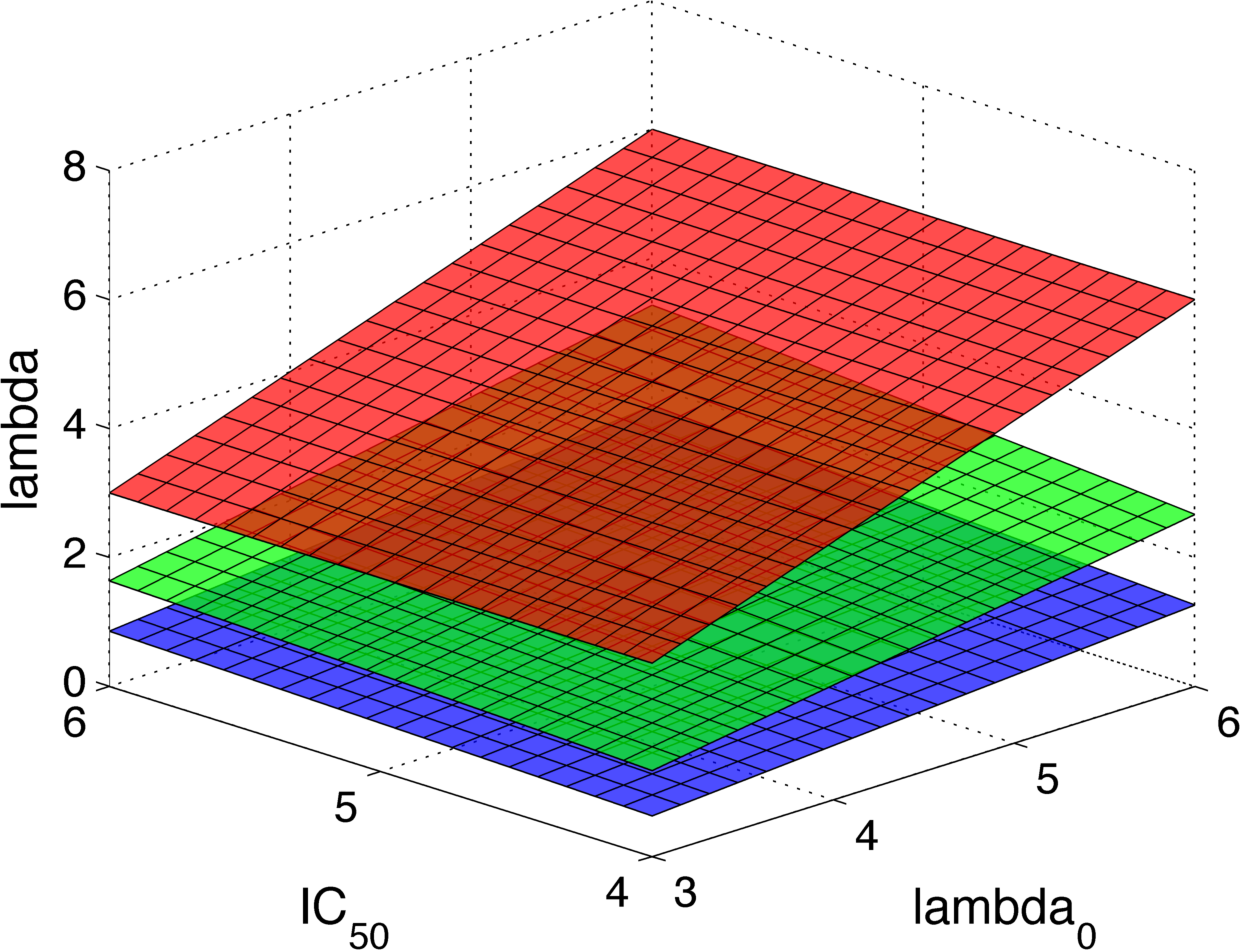
\includegraphics[width=.45\textwidth]{pics/CTS4_lambda_threeSurfaces} & 
\raisebox{0\height}{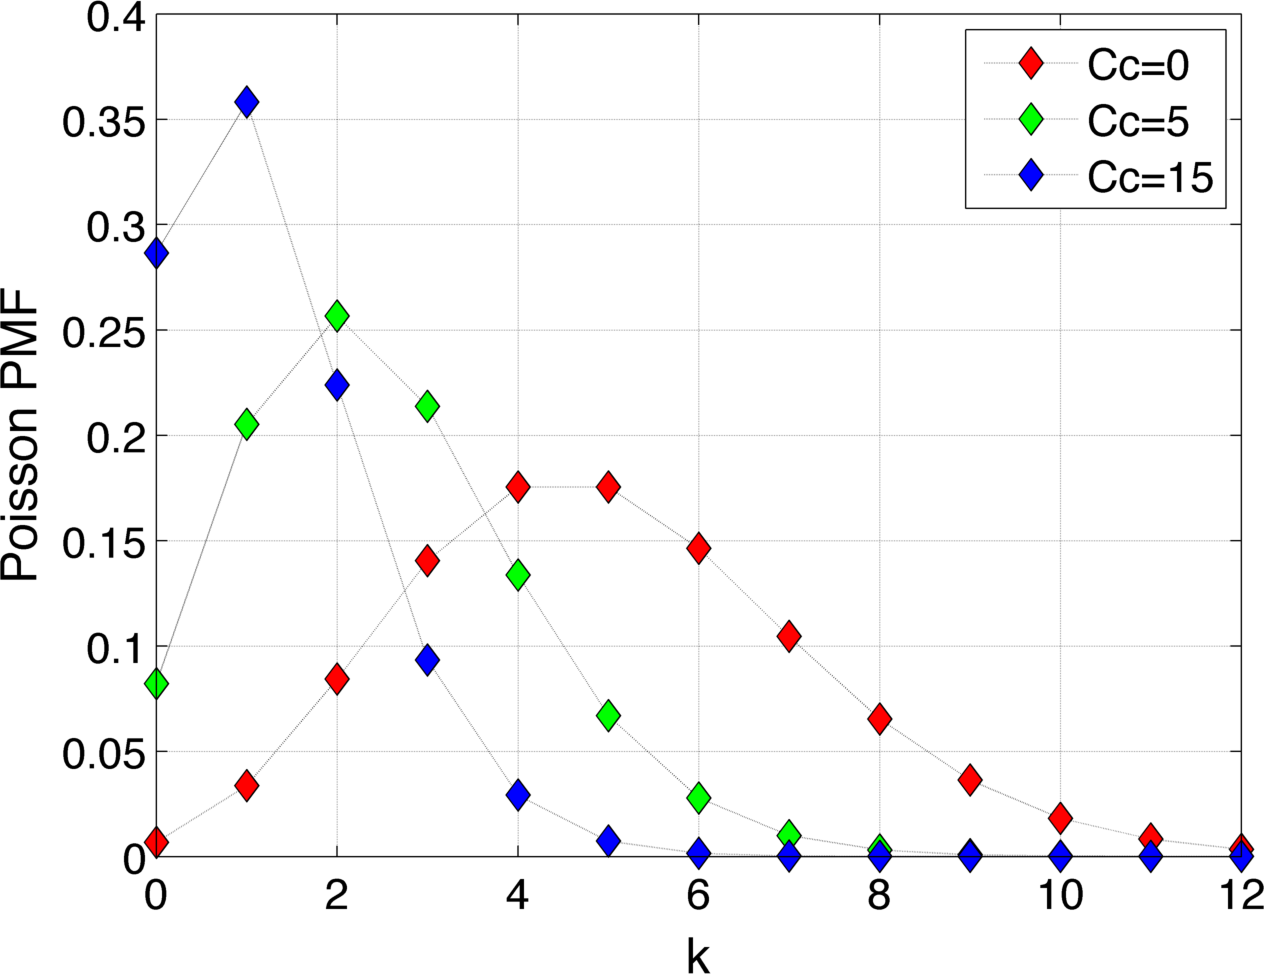
\includegraphics[scale=0.45]{pics/CTS4_poissonScan}}
\end{tabular}
\caption{(LEFT) $\lambda$--surface as function of $\lambda0$ and $IC50$ plotted for $Cc = \{1,5,15\}$. (RIGHT) Poisson PMF for fixed parameters $\lambda0 = IC50 = 5$ and varying concentration $Cc = \{1,5,15\}$.}
\label{fig:lambdasurface}
\end{figure}


%%%%%%%%%%%%%%%%%%%%%%%%%%%%%%%%%%%%%%%%%%%%%%%%%%%%%%%%%%%%%%%%
\subsubsection{Model description}
\label{subsec:exp5_TaskDescription}

%\paragraph{Individual parameters model}
%
%Details omitted here...
%
%\begin{eqnarray}
%ka& \sim& \mbox{logNormal}(ka_{\rm pop}, \omega_{ka});  \quad ka_{\rm pop}=1,\quad \omega_{ka}=0.6 \nonumber \\
%V& \sim& \mbox{logNormal}(V_{\rm pop}, \omega_{V}); \quad V_{\rm pop}=8,\quad \omega_V=0.2 \nonumber \\
%CL& \sim&  \mbox{logNormal}(CL_{\rm pop}, \omega_{CL}); \quad CL_{\rm pop}=0.13,\quad \omega_{CL}=0.2 \nonumber \\
%\lambda0 & \sim&  \mbox{logNormal}(\lambda0_{{\rm pop}}, \omega_{\lambda0}); \quad  \lambda0_{{\rm pop}} = 5, \quad \omega_{\lambda0} = 0.2 \nonumber \\
%IC50 &\sim& \mbox{logNormal}(IC50_{{\rm pop}}, \omega_{IC50}); \quad  IC50_{{\rm pop}} = 5, \quad \omega_{IC50} = 0 \nonumber
%\end{eqnarray}
%\begin{eqnarray}
%\log(V_i) &=& \log(V_{pop}) + \beta_{1,V}\log(W_i/70) + \eta_{V,i} \nonumber \\
%\log(CL_i) &=& \log(CL_{pop}) + \beta_{1,CL}\log(W_i/70) + \eta_{CL,i} \nonumber \\
%\beta_{1,V}&=&1 \nonumber \\
%\beta_{1,CL}&=&0.75 \nonumber \\
%\rho_{V,CL}&=&0.7 \mbox{  (the correlation coefficient between } \eta_{V,i} \mbox{ and } \eta_{CL,i}  \mbox{)} \nonumber
%\end{eqnarray}


\paragraph{Structural model}
\begin{eqnarray}
\frac{dAd}{dt} &=&-ka \times Ad \nonumber \\
\frac{dAc}{dt}&=&ka \times Ad - k \times Ac \nonumber \\ 
Cc &=& Ac/V \nonumber \\ \nonumber
\end{eqnarray}
\paragraph{Observation model}

\begin{itemize}
\item
Data type: discrete/count 
\item
Count variable: $Y$
\item
log(Poisson PMF)
\begin{align}
& Log(P(Y=k)) = -\lambda + k\times log(\lambda) - \log(k!) \nonumber
\end{align}
\item
Rate parameter $\lambda$, the Poisson 'intensity' is function of drug concentration, $Cc$
\begin{align}
& \lambda = \lambda0 (1 - Cc/(IC50 + Cc)) \nonumber
\end{align}
\end{itemize}

\subsubsection{PharmML code}
The code below covers the Observation model with eqs.(\ref{eq:logPMF}) and (\ref{eq:lambda}).
All parameters are assumed to be defined in the \xelem{ParameterModel}.
\lstset{language=XML}
\begin{lstlisting}
        <ObservationModel blkId="om1">
            <Discrete>
                <CountData>
                    <CountVariable symbId="k"/>
                    
                    <!-- Poisson intensity - function of drug concentration, Cc -->                    
                    <IntensityParameter symbId="Lambda">
                        <ct:Assign>
                            <math:Equation>
                                <math:Binop op="times">
                                    <ct:SymbRef blkIdRef="pm1" symbIdRef="lambda0"/>
                                    <math:Binop op="minus">
                                        <ct:Real>1</ct:Real>
                                        <math:Binop op="divide">
                                            <ct:SymbRef blkIdRef="sm1" symbIdRef="Cc"/>
                                            <math:Binop op="plus">
                                                <ct:SymbRef blkIdRef="pm1" symbIdRef="IC50"/>
                                                <ct:SymbRef blkIdRef="sm1" symbIdRef="Cc"/>
                                            </math:Binop>
                                        </math:Binop>
                                    </math:Binop>
                                </math:Binop>
                            </math:Equation>
                        </ct:Assign>
                    </IntensityParameter>
                    
                    <!-- log(P(Y=k)) = -lambda+k*log(lambda)-log(k!) -->
                    <PMF linkFunction="log">
                        <math:LogicBinop op="eq">
                            <ct:SymbRef symbIdRef="Y"/>
                            <ct:SymbRef symbIdRef="k"/>
                        </math:LogicBinop>
                        <PoissonDistribution xmlns="http://www.uncertml.org/3.0" 
                            definition="http://www.uncertml.org/3.0">
                            <rate>
                                <var varId="Lambda"/>
                            </rate>
                        </PoissonDistribution>
                    </PMF>
                </CountData>
            </Discrete>
        </ObservationModel>
\end{lstlisting}






%\subsubsection{Poisson model}
%
%\subsubsection{NM-TRAN code provided by Nick Holford and Mike Smith}
%\begin{lstlisting}
%$PROB Count data
%$DATA ..\count_sim.std\count_sim.fit IGNORE @
%$INPUT ID TIME CMTX AMT RATX WT AGE SEX TYPE CP DV MDV
%;$SIM (20000321 NEW) (1234567 UNIFORM) SUBPROBLEMS=1
%$ESTIM MAXEVAL=9990 METHOD=COND LAPLACE -2LL NOABORT
% 
%$THETA
% 
%(0,1) FIX    ; pop_cl
%(1,10) FIX ; pop_v
%(0,0.5) FIX ; pop_ka
%(0,10,)      ; BaseCount
%(0,.5,10)    ; Beta
% 
%$OMEGA
%0.09 FIX ; ppv_cl
%0.09 FIX ; ppv_v
%0.09 FIX ; ppv_ka
%0.04 ; ppv_event
% 
%$SUBROUTINE ADVAN=2 TRAN=2
% 
%$PK
%     GRPCL  = POP_CL
%     GRPV   = POP_V
%     GRPKA  = POP_KA
%     
%     PPVCL  = PPV_CL
%     PPVV   = PPV_V
%     PPVKA  = PPV_KA
% 
%     CL     = GRPCL*EXP(PPVCL)
%     V      = GRPV*EXP(PPVV)
%     KA     = GRPKA*EXP(PPVKA)
%      
%     S2     = V
%     REPI   = IREP
%      
%$ERROR
%; Drug effect
% 
%COUNT=BaseCount + Beta*CP + ppv_event
% 
%;Stirlings formula for log DV factorial
%IF (DV.GT.0) THEN
%      LDVFAC=(DV+.5)*LOG(DV)-DV+.5*LOG(6.283185)
%ELSE
%      LDVFAC=0
%ENDIF
% 
%Y=-2*(-COUNT+DV*LOG(COUNT)-LDVFAC)
% 
%;$TABLE ID TIME CMTX AMT RATX WT AGE SEX TYPE CP MDV COUNT
%;NOPRINT FILE=count.fit
%\end{lstlisting}



%\subsubsection{Poisson model - P}
%\paragraph{NM-TRAN code provided by Elodie Plan}
%\begin{lstlisting}
%\end{lstlisting}
%\paragraph{MLXTRAN code from Monolix 4.1 User Manual}
%\begin{lstlisting}
%\end{lstlisting}
%
%
%\begin{sidewaystable}[h]
%\caption{Performance After Post Filtering}  % title name of the table
%\centering  % centering table
%\begin{tabular}{l c c rrrrrrr}  % creating 10 columns
%\hline\hline                       % inserting double-line
% Audio &Audibility & Decision &\multicolumn{7}{c}{Sum of Extracted Bits} 
%\\ [0.5ex]   
%\hline              % inserts single-line
%% Entering 1st row
% & &soft &1 & $-1$ & 1 & 1 & $-1$ & $-1$ & 1  \\[-1ex]
%\raisebox{1.5ex}{Police} & \raisebox{1.5ex}{5}&hard
%&  2 & $-4$ & 4 & 4 & $-2$ & $-4$ & 4 \\[1ex]
%% Entering 2nd row
%& &soft & 1 & $-1$ & 1 & 1 & $-1$ & $-1$ & 1  \\[-1ex]
%\raisebox{1.5ex}{Beethoven} & \raisebox{1.5ex}{5}& hard
%&8 & $-8$ & 2 & 8 & $-8$ & $-8$ & 6 \\[1ex]
%% Entering 3rd row
%& &soft & 1 & $-1$ & 1 & 1 & $-1$ & $-1$ & 1  \\[-1ex]
%\raisebox{1.5ex}{Metallica} & \raisebox{1.5ex}{5}& hard
%&4 & $-8$ & 8 & 4 & $-8$ & $-8$ & 8  \\[1ex]
%% [1ex] adds vertical space
%\hline                          % inserts single-line
%\end{tabular}
%\label{tab:LPer}
%\end{sidewaystable}
%
